\section{Using policy languages to specify access conditions}
\label{sec:sota_policies}

Policy languages have been used in the last decades to specify information regarding the usage of data, e.g., to represent licenses associated with datasets or software usage.
As such, they seem perfectly aligned with the goal of representing the conditions to access data on the Web, whether being preferences set by data subjects or access requests from other entities.
In addition, if used together with privacy and data protection-specific terms, e.g., coming from the ontologies described in the previous Section, they can be used to model legally-aligned access control policies.

In the following Sections, the criteria used to analyse each specified policy language are described, as well as a description of each identified language.

\subsection{Criteria for analysis}
\label{sec:sota_policies_criteria}

Each solution is accompanied by an introductory summary of the language, detailing its primary contributions, followed by an overview of its core elements.
Additionally, where applicable, specific examples of use cases employing the language are provided, along with details on any derived implementations, including information on available reasoners that use it.
The dependencies on prior existing works are also noted when outlined in the literature.
Table~\ref{tab:resources-policy-languages} presents a concise description of the policy languages detailed in the following Sections, along with details about the creators of the resources, version number, publication date, and the most recent update date.
The solutions were examined chronologically based on their publication date, followed by their last update date.
Figure~\ref{fig:lang-dependency-graph} depicts a dependency graph illustrating the relationships between languages, their dependencies, and subsequent developments.

\begin{table}[ht]
\centering
\caption{Brief description of the policy languages described in Section \ref{sec:sota_policies_description}.}
\label{tab:resources-policy-languages}
\resizebox{\textwidth}{!}{%
\begin{tabular}{c||c|c|c|c|c}
Abbreviation (Section) & Full Name & Creators & Version & \multicolumn{1}{c|}{\begin{tabular}[c]{@{}c@{}} Date of \\ publication \end{tabular}} & \multicolumn{1}{c}{\begin{tabular}[c]{@{}c@{}} Last \\ update \end{tabular}} \\
 \hline\hline
 P3P (\ref{sec:p3p}) & Platform for Privacy Preferences & Cranor et al. & 1.0 & 1998 & 2010 \\
 \hline
 ODRL (\ref{sec:odrl}) & Open Digital Rights Language & Iannella et al. & 2.2 & 2001 & 2019 \\
 \hline
 XPref (\ref{sec:xpref}) & XPath-based Preference Language & Agrawal et al. & - & 2003 & - \\
 \hline
 AIR (\ref{sec:air}) & Accountability In RDF & Khandelwal et al. & - & 2007 & 2009 \\
 \hline
 S4P (\ref{sec:s4p}) & SecPAL for Privacy & Becker et al. & - & 2009 & 2010 \\
 \hline
 POL (\ref{sec:pol}) & Privacy Option Language & Stefan Berthold & - & 2010 & 2013 \\
 \hline
 PPO (\ref{sec:ppo})& Privacy Preference Ontology & Sacco and Passant & - & 2011 & 2013 \\
 \hline
 LegalRuleML (\ref{sec:legalruleml}) & LegalRuleML Core Specification & Palmirani et al. & 1.0 & 2012 & 2021 \\
 \hline
 A-PPL (\ref{sec:appl}) & Accountable Policy Language & Azraoui et al. & - & 2013 & 2016 \\
 \hline
 P2U (\ref{sec:p2u}) & Purpose-To-Use & Iyilade and Vassileva & - & 2014 & - \\
 \hline
 SPL (\ref{sec:special}) & SPECIAL Usage Policy Language & Bonatti et al. & 1.0 & 2017 & 2019 \\
 \hline
 DPF (\ref{sec:dpf}) & Declarative Policy Framework & Martiny et al. & - & 2018 & 2020 \\
 \hline
 LPL (\ref{sec:lpl}) & Layered Privacy Language & Gerl et al. & - & 2018 & 2019 \\
\end{tabular}}
\end{table}

\begin{figure}
    \caption{Privacy-related policy languages dependency chart.}
    \label{fig:lang-dependency-graph}
    \centering
    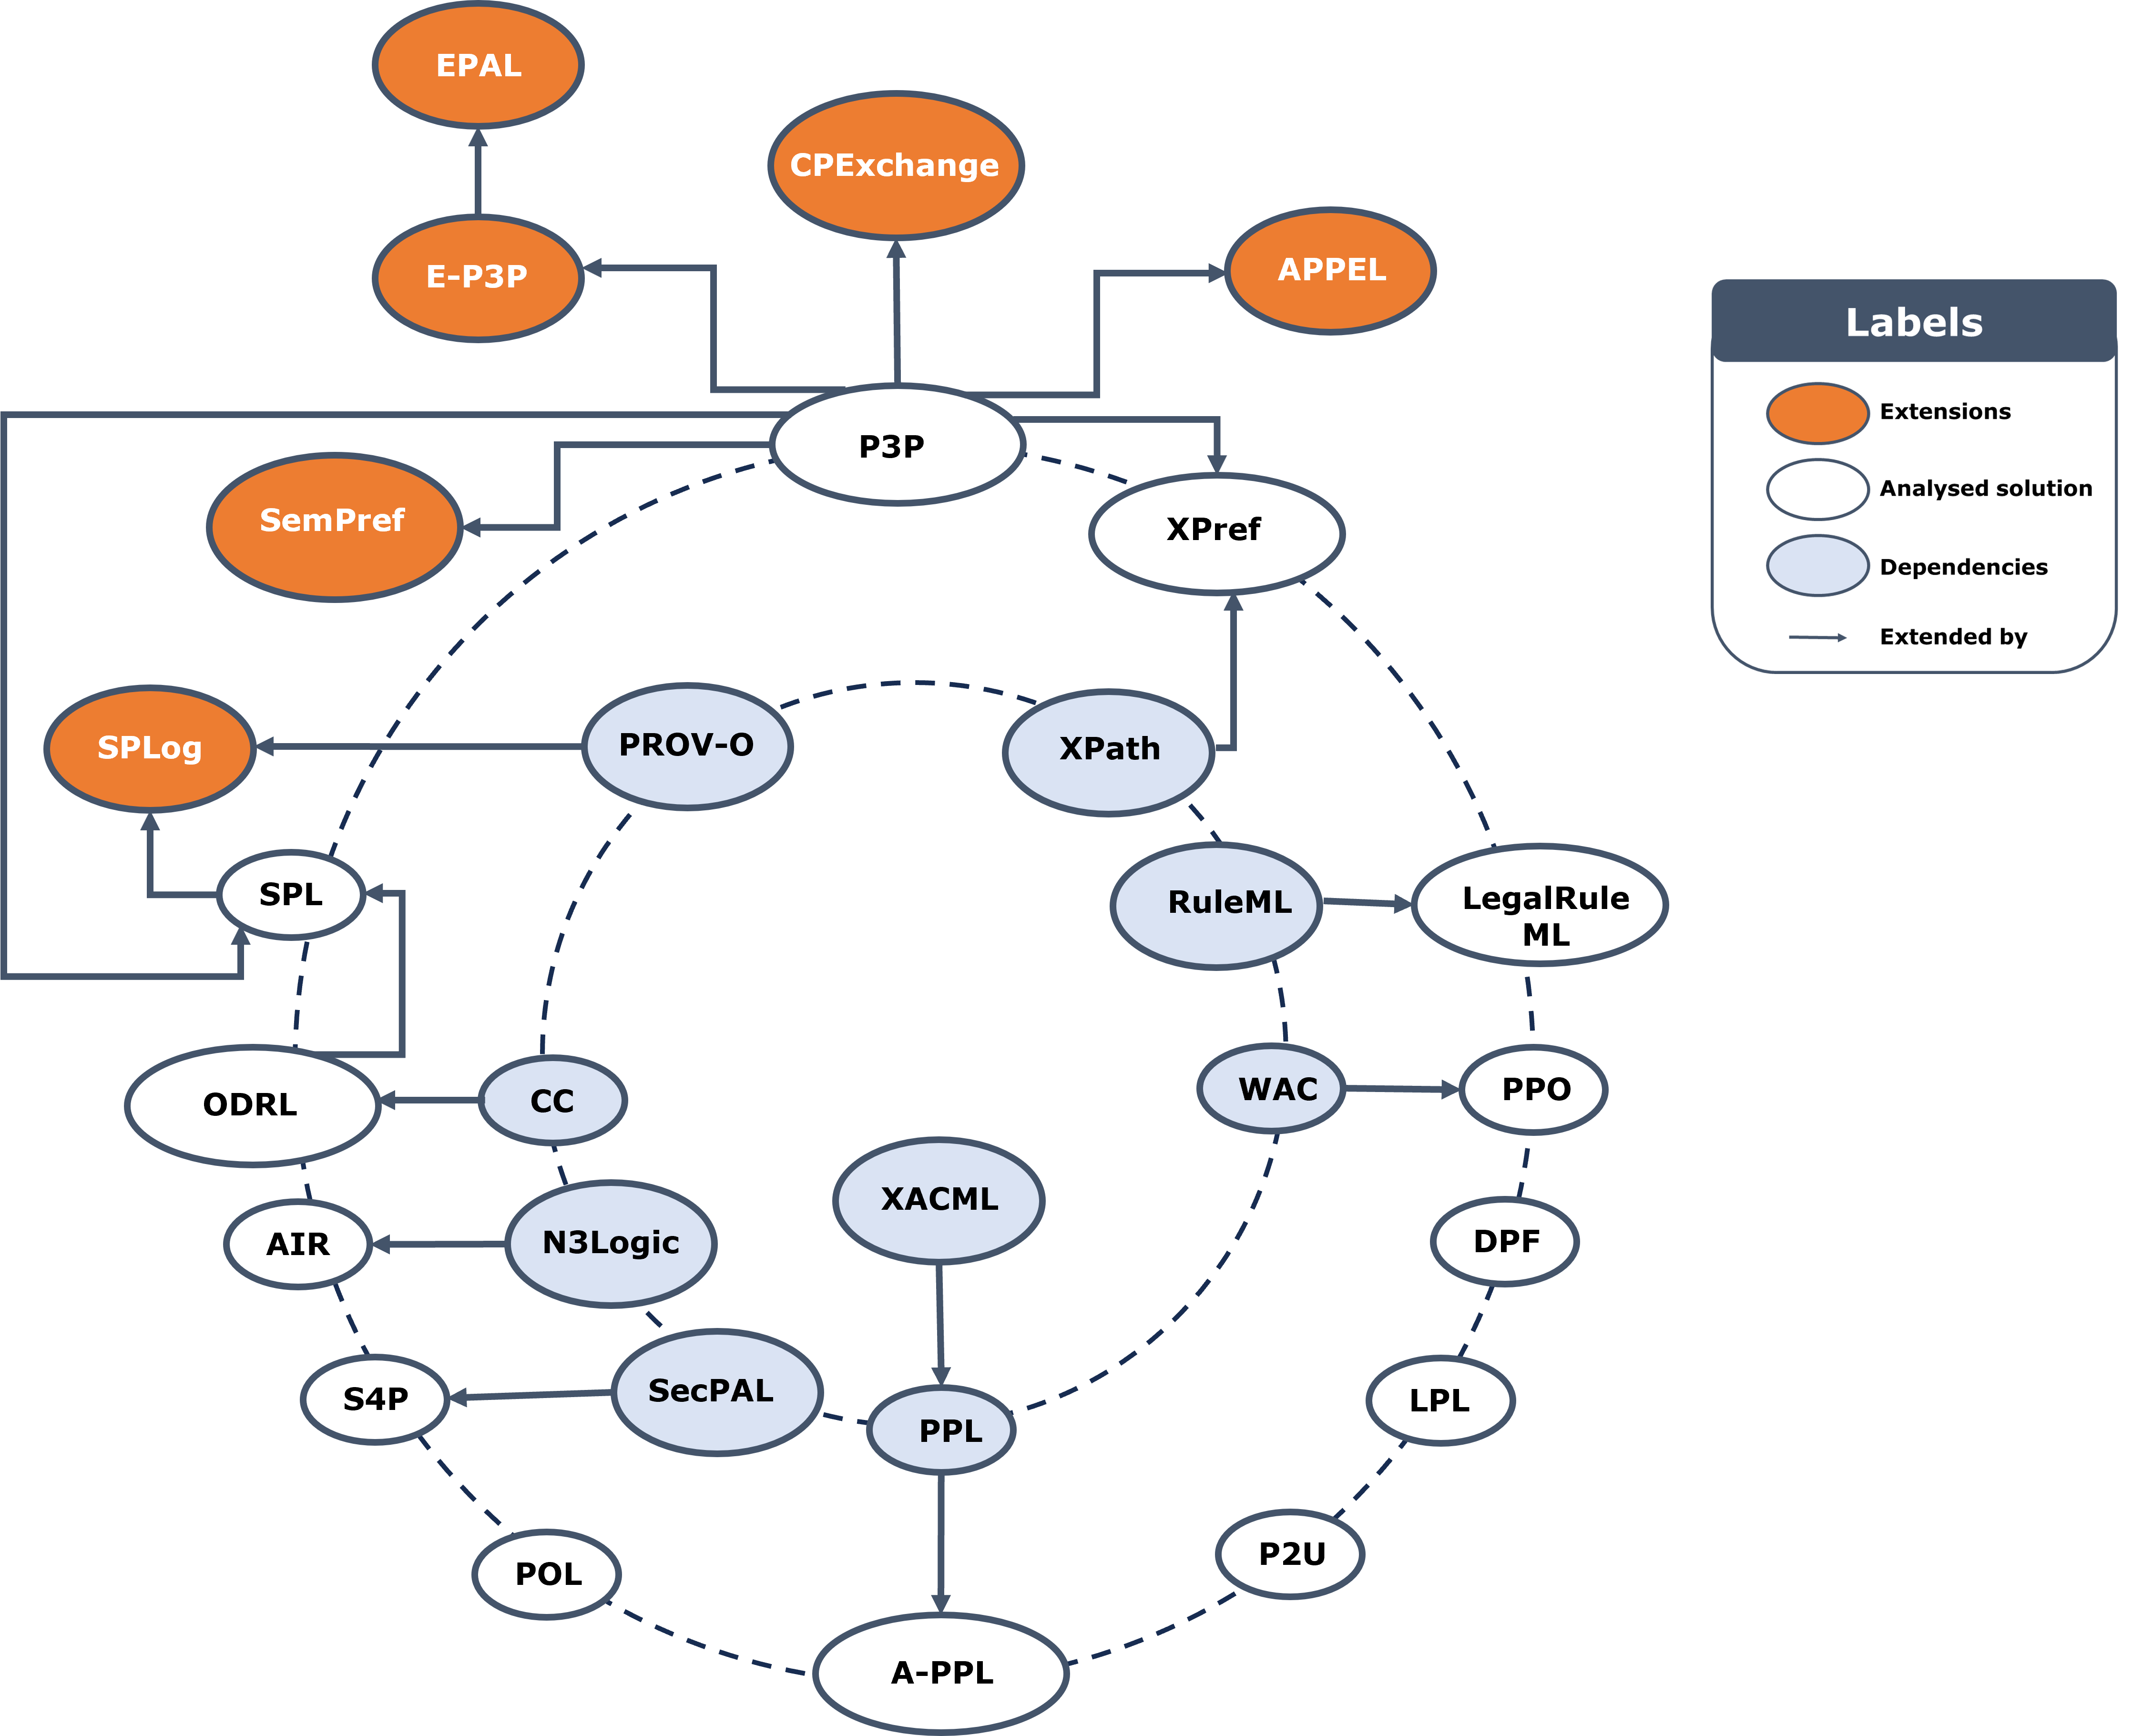
\includegraphics[width=\textwidth]{figures/chapter-2/languages.png}
\end{figure}

Moreover, the following criteria were used to analyse existing research on semantic policy languages:
\begin{enumerate}
    \item[(C1)] Ability to model deontic concepts, e.g., permissions, prohibitions, obligations.
    \item[(C2)] Ability to model GDPR concepts, such as the privacy terms in Table \ref{tab:GDPR_privacy_terms}.
    \item[(C3)] Existence of taxonomies of terms to populate policy conditions.
    \item[(C4)] Existence of mechanisms to assist with compliance.
    \item[(C5)] Resource is maintained/continues to be actively developed.
    \item[(C6)] Existence of an open and accessible specification.
\end{enumerate}

The outcomes of this comparative analysis will be provided in Section~\ref{sec:sota_policies_analysis} and systematised in Table~\ref{tab:languagesComparison}.

\subsection{Semantic policy languages for access control}
\label{sec:sota_policies_description}

This Section's main goal is to describe existing policy languages related to privacy, delineating the structure and information offered by each language.
Additionally, their compatibility with the GDPR is assessed, focusing on their ability to describe the provisioned rights and obligations.
Moreover, Table~\ref{tab:resources-policy-languages} provides an overview of these languages and collects information about the creators of the resources, their versions, the date of publication, and the date of the last known update.
Said languages are then analysed in chronological order regarding the date of publication and a dependency graph is presented in Figure~\ref{fig:lang-dependency-graph}.

To complement the description of the languages presented in this Section, additional documentation and resources were published on a Web page\footnote{Available at \url{https://w3id.org/people/besteves/phd/sota/languages}. Its public repository can be consulted at \url{https://w3id.org/people/besteves/phd/sota/repo} for further improvement when new solutions appear.}, including diagrams and code examples.

\subsubsection{P3P}
\label{sec:p3p}

\cite{cranor_platform_2002} introduced the Platform for Privacy Preferences (P3P) language as a standard for Web services to disclose their privacy practices in a machine-readable format.
This facilitated user agents in easily interpreting these practices and notifying users about decisions based on them. 
However, despite enabling users to be informed about the privacy policies of Web pages, these mechanisms do not ensure that the pages are actively adhering to these policies, as P3P lacks enforcement capabilities.
Therefore, the P3P vocabulary was designed not to comply with a specific regulation but rather to specify the practices of single Web pages.

The primary contributions of the P3P specification include a data schema for outlining the data intended to be collected by the Web page, a standardised set of purposes, data categories, and recipients, and an XML standard for defining privacy policies.
P3P policies consist of both general assertions and specific statements, the latter being related only to certain types of data.
General assertions encompass the legal entity applying the policy and informational elements related to access, disputes, and remedies.
The access element indicates whether the Web page allows access to the data it gathers and the disputes element outlines a process for resolving privacy-related disputes, while the remedy element details potential solutions in the event of a policy breach.
Additionally, each P3P statement consists of a distinct `data group' containing one or more data elements, along with purpose, recipient types, and retention elements.
In this context, P3P outlines a range of purposes relevant to Web-based data processing operations, such as facilitating and supporting the initial activity for which the data was supplied, conducting research and development, or performing data analysis.
%The purpose element is required to include at least one specification of purpose.
The recipient type element can be used to specify who will benefit from the collected data, while the retention element must accurately reflect the policy regarding how long the data will be kept.
Listing~\ref{list:p3p_example} displays a P3P policy that underscores the aforementioned P3P elements.
CatalogExample gathers essential details concerning its users' computer systems, as well as data regarding the pages they visit.
This information serves system administration and research and development purposes and is exclusively utilised by the company and retained for a duration deemed suitable for the specified purposes.

\begin{listing}
\caption{P3P policy extracted from Example 3.1 of the P3P specification~\citep{cranor_platform_2002}, which specifies the privacy policy of CatalogExample.}
\label{list:p3p_example}
\begin{minted}{turtle}
<http://example.com/#forBrowsers> a p3p:Policy ;
    p3p:disclosure <http://example.com/PrivacyPractice.html> ;
    p3p:entity [
        p3p:business.name [ rdf:value "CatalogExample" ] ;
        p3p:business.contact-info.postal.street [
            rdf:value "4000 Lincoln Ave." ] ;
        p3p:business.contact-info.postal.city [
            rdf:value "Birmingham" ] ;
        p3p:business.contact-info.postal.stateprov [ rdf:value "MI" ] ;
        p3p:business.contact-info.postal.country [ rdf:value "USA" ] ;
        p3p:contact.online.email [ rdf:value "catalog@example.com" ] ;
        p3p:contact.telephonenum.intcode [ rdf:value "1" ] ;
        p3p:contact.telephonenum.loccode [ rdf:value "248" ] ;
        p3p:contact.telephonnum.number [ rdf:value "3926753" ] ] ;
    p3p:access p3p:AccessClass-nonident ;
    p3p:statement [
        p3p:purposeAlways p3p:Purpose-admin, p3p:Purpose-develop ;
        p3p:recipientAlways p3p:Recipient-ours ;
        p3p:retention p3p:Retention-stated-purpose ;
        p3p:data [
            rdf:predicate p3p:dynamic.clickstream, p3p:dynamic.http ] ] .
\end{minted}
\end{listing}

P3P was initially developed to articulate policies of Web services, prompting the design of APPEL as an extension to empower users in expressing their preferences~\citep{cranor_p3p_2002}.
Consequently, the utilisation of both languages becomes imperative to align user privacy preferences with service privacy policies.
Furthermore, \cite{bohrer_customer_2000} introduced the CPExchange language, an XML specification facilitating the transfer of customer data across enterprise services, incorporating P3P privacy policies relevant to the exchanged data.
Likewise, EPAL~\citep{ashley_enterprise_2003}, developed by IBM Research\footnote{\url{http://www.research.ibm.com/} (accessed on 16/July/2023)} along with its precursor E-P3P~\citep{ashley_e-p3p_2002}, leveraged P3P statements to align enterprise privacy policies with user preferences.
\cite{li_semantics-base_2006} introduces a declarative data-centric semantic model alongside a succinct syntax for P3P policies, facilitating the representation of the relationship between various P3P elements.
The primary aim of this language is to articulate policies in a manner that can be uniformly interpreted and represented across diverse user agents.
Extending this semantic foundation, the authors put forward SemPref, a preference language that considers the significance of the privacy policy rather than its syntactic form.

The P3P 1.0 Specification achieved W3C Recommendation status on April 16, 2002.
Nonetheless, its adoption was restricted as it requires acceptance from both Web services and users.
Furthermore, there has been no protocol established for these P3P policies to accurately reflect the privacy practices of Web pages.
While this specification did attain W3C recommendation status, its failure to gain widespread adoption rendered it obsolete by 2018.
Nonetheless, the significance of P3P remains considerable, as its inception and utilisation marked a pioneering endeavour in the realm of machine-readable privacy languages. 
Consequently, the primary lessons derived from this language pertain to the necessity of establishing a formal semantics capable of delineating both data subject and controller policies, which accurately reflect their data preferences and practices, and the need for tools that effectively enforce the outlined policies.

\subsubsection{ODRL}
\label{sec:odrl}

The ODRL Vocabulary \& Expression 2.2~\citep{iannella_odrl_2018} gained W3C Recommendation status in February 2018, developed by the Permissions \& Obligations Expression Working Group, with its initial version launched back in 2001.
Its primary objective was to establish a language capable of translating natural language policies into machine-readable formats, specifying details regarding permissions, prohibitions, and obligations pertaining to an asset.
This vocabulary stems from the consolidation of previous efforts undertaken by the ODRL CG, encompassing the ODRL V2.1 Common Vocabulary, the ODRL V2.1 XML Encoding, the ODRL V2.1 Ontology, and the ODRL V2.1 JSON Encoding.
Ongoing maintenance of the ODRL's standards and specifications are supported by the ODRL CG.

ODRL includes two vocabularies for the description of policies: the ODRL Core Vocabulary and the ODRL Common Vocabulary.
The primary class within ODRL's Core Vocabulary is the `policy' concept, facilitating the identification of a specific policy through its unique identifier.
Within each policy, there may exist multiple rules -- an abstract class that outlines the shared characteristics of permissions, prohibitions, and duties.
These rule types serve to declare whether a particular action, e.g., over as asset, is permitted, prohibited, or obligatory.
Additionally, permissions might also be linked with duties that must be fulfilled for said permissions to be active.
Furthermore, rules undergo further refinement through the usage of constraints, which specify the circumstances under which the rule applies, e.g., a particular permission remains valid until the conclusion of 2024.
The ODRL Vocabulary also outlines a collection of 49 actions, nine of which are imported the Creative Commons (CC) vocabulary.
The entities, or parties, involved (which can encompass a group of individuals, an organisation, or an agent) are responsible for enforcing the rules and may assume various roles contingent upon their relationship with the asset, e.g., the entity issuing the rule adopts the assigner role, whereas the recipient of the rule assumes the assignee role.
An asset, on the other hand, refers to an identifiable resource, such as data, software, services, or a combination thereof, that is subject to a rule.
The ODRL Common Vocabulary further delineates subclasses of policies, roles played by the involved parties, taxonomies of use and transfer actions for rules, and a variety of constraint operands, such as temporal, spatial, or sector-specific.
Of particular significance concerning the GDPR is the privacy policy subclass regarding assets containing personal data. 
Consequently, privacy policies implementing the ODRL language must specify to the involved parties the manner in which data is utilised, as well as with whom and for what purpose.
Listing~\ref{list:odrl_example} provides an implementation of an ODRL privacy policy that underscores the aforementioned elements, including a duty for the assignee to be allowed to use the data and a consequence in case they do not.

\begin{listing}
\caption{ODRL \texttt{Privacy} policy.}
\label{list:odrl_example}
\begin{minted}{turtle}
<http://example.com/privacy-policy> a odrl:Privacy ;
    odrl:uid <http://example.com/privacy-policy> ;
    odrl:permission [
        odrl:target <http://example.com/beatriz/contacts> ;
        odrl:assignee <http://example.com/beatriz> ;
        odrl:assigner <http://example.com/company-a> ;
        odrl:action odrl:use ;
        odrl:duty [
            odrl:action odrl:obtainConsent ;
            odrl:consentingParty <http://example.com/beatriz> ;
            odrl:consequence [
                odrl:assigner <http://example.com/company-a> ;
                odrl:action odrl:delete ] ] ] . 
\end{minted}
\end{listing}

ODRL's representational capabilities exhibit some limitations, as highlighted by~\cite{kebede_critical_2020}, particularly regarding the portrayal of delegation, the various semantics utilised for expressing duties, and the management of conflicts.
Nevertheless, efforts such as those described by~\cite{fornara_operational_2018, fornara_using_2019} are underway to formalise the semantics of ODRL policies.

ODRL was applied in various contexts, including its usage by working groups within the Open Mobile Alliance SpecWorks\footnote{\url{https://www.omaspecworks.org/} (accessed on 18/July/2023)} and by the IPTC Rights Expressions WG for the RightsML Standard\footnote{\url{https://www.iptc.org/std/RightsML/2.0/RightsML_2.0-specification.html} (accessed on 18/July/2023)}.

\subsubsection{XPref}
\label{sec:xpref}

\cite{agrawal_xpref_2005} introduced XPref as an alternative to APPEL, which only permits the definition of P3P policies that are not allowed by the user.
XPref utilises XPath (XML Path Language) 1.0 and 2.0 expressions to replace APPEL rules, enhancing the precision and reducing errors in policy formulation.
Both XPath 1.0, as described by~\cite{clark_xml_1999}, and XPath 2.0, as detailed by~\cite{berglund_xml_2010}, attained W3C Recommendation status on November 16th, 1999, and December 14th, 2010, respectively.
It should be noted that these specifications are no longer subject to further maintenance since subsequent versions have been developed.
In this context, the primary objective of XPath is to offer a method for traversing the hierarchical elements within an XML document.
In pursuit of this objective, XPath views an XML document as a tree structure of nodes
When an XPath expression is applied to the document, it determines an ordered sequence of nodes, resulting in a concise path representation.
This path consists of expressions that yield various types of nodes, including root, element, text, attribute, namespace, processing instruction, or comment nodes.

XPref was crafted to ensure that its rules not only recognise combinations of P3P elements that render a policy unacceptable based on user preferences, but also confirm that the presented elements are defined as acceptable.
It achieves these objectives while preserving the syntax and semantics of APPEL, along with its core classes.
However, the contents of the rules are substituted with XPath expressions, given that P3P policies are XML documents and can thus be readily compared with XPath-based rules.
These expressions are defined by appending a `condition' attribute to the rule, which activates the rule when the XPath expression yields a non-empty result.
%Consequently, utilising the `behavior' attribute in XPref rules allows for preferences to be set to either permit or restrict services based on the P3P policy elements they contain, such as purposes and recipients, specified in the "condition" attribute.

\subsubsection{AIR}
\label{sec:air}

In 2010, \citeauthor{hitzler_analyzing_2010} developed Accountability in RDF (AIR) -- a declarative language enabling the assertion of facts and the inclusion of rules.
AIR is built on N3Logic~\citep{berners-lee_n3logic_2008}, which supports rule nesting, rule reuse, and automated explanations of actions carried out by the AIR reasoner. 
These explanations can be customised and, given that they may contain sensitive data like Personally Identifiable Information (PII), can be employed to ensure privacy.
For example, they can be utilised to conceal actions executed under specific rules.

N3Logic extends the RDF data model with the aim of expressing logic rules on the Web, thereby promoting the use of a unified language for both data representation and logical inference.
Thus, AIR leverages N3Logic's inherent capabilities, including built-in functions, nested graphs, and contextualised reasoning.
This enables AIR rules to incorporate the usage of graphs as literal values, and built-in functions or operators defined as RDF properties.

Each AIR rule is assigned a unique IRI, ensuring its seamless integration with the linked data cloud and facilitating its reuse.
These rules adhere to the following structure: \texttt{air:if} \texttt{condition}; \texttt{air:then} \texttt{then-actions}; \texttt{air:else} \texttt{else-actions}.
The action instances can include annotations using the \texttt{air:description} property.
These annotations are subsequently integrated by the AIR reasoner into its justifications and can serve to conceal PII found within the rules.
Additionally, the format of the rules graph permits the nesting of rules within the same rule set.
This feature offers a means to segment the conditions outlined by the rule, allowing only a portion of them to be revealed in the justifications.

\subsubsection{S4P}
\label{sec:s4p}

S4P (SecPAL for Privacy), designed by \cite{becker_framework_2009, becker_s4p_2010}, constitutes a language framework designed for articulating users' privacy preferences and the data handling practices of Web services. Originating from Microsoft Research\footnote{\url{https://www.microsoft.com/en-us/research/} (accessed on 16 March 2024)}, this language serves as an extension of the company's earlier endeavor, SecPAL, aimed at delineating PII management.

SecPAL \citep{becker_design_2007} is a flexible, decentralised authorisation language, crafted for articulating policies and enhancing their expressiveness to define delegation conditions, domain-specific constraints, and negation.
An authorisation policy comprises a set of assertions, each associated with an issuer responsible for vouching for the assertion, along with a collection of conditional facts and constraints pertaining to temporal or spatial aspects.
Subsequently, when an access request is made, it undergoes a transformation into a series of queries.
These queries are then matched against the clauses that represent the system's policies, ultimately leading to a decision on data access conditions.
S4P extends SecPAL by treating granted rights and required obligations as assertions and queries.
Based on these, a satisfaction checking algorithm is formulated to evaluate the disclosure of PII between users and data-collecting services.
As a result, services should articulate their data-handling practices in the form of SecPAL queries.
Conversely, users specify their preferences as SecPAL assertions, precisely delineating what services are authorised to do and what duties they have regarding r=the usage of said PII.
% The satisfaction algorithm evaluates whether the data collection practices of the services align with the behaviors permitted by the users and whether the obligations specified in the users' preferences are adhered to by the services' policies.
If the algorithm yields a positive result, indicating that the service's policies complies with the user's preferences, the service can proceed with its data handling activities.
Additionally, S4P establishes a data disclosure protocol to ensure that users' preferences are respected when their data is shared with third party recipients.
% This protocol permits the disclosure of the user's PII only if the service's policies satisfy the user's preferences and if the policies of the third parties are in harmony with the user's preferences.

In addition to possessing an XML schema for implementation purposes, S4P features a human-readable and unambiguous syntax, enabling its utilisation in various applications. 
Listing~\ref{list:s4p_example} illustrates the S4P syntax in a scenario where Alice, the user, delineates her privacy preferences concerning the collection of her email address. 
Specifically, Alice permits eBooking services to utilise her email address for sending confirmations, newsletters, and for statistical purposes.
Additionally, Alice authorises the booking services to share her email address with trusted partners exclusively to engage with registered services that commit to deleting her email address within a month.

\begin{listing}
\caption{S4P example, extracted from \cite{becker_framework_2009}, which specifies Alice's privacy preferences concerning the collection of her email address by eBooking services.}
\label{list:s4p_example}
\begin{minted}[escapeinside=||]{python}
Alice says x may use Email for p if
    x is a eBookingService,
    where p |$\in$| {Confirmation, Newsletter, Stats}
Alice says x may send Email to y if
    x is a eBookingService,
    y is a TrustedPartner
Alice says x can say y is a TrustedPartner if
    x is a eBookingService
Alice says |$\langle$|Service|$\rangle$| is a RegisteredService|$?$| |$\wedge$|
    |$\exists$|t (|$\langle$|Service|$\rangle$| says |$\langle$|Service|$\rangle$| will delete Email within t|$?$| |$\wedge$| t |$\leq$| 30 days|$?$|)
\end{minted}
\end{listing}

\subsubsection{POL}
\label{sec:pol}

The Privacy Option Language (POL) was formulated by~\cite{berthold_privacy_2013} to establish privacy contracts between data controllers and data subjects, drawing on the principles of financial option contracts and corresponding data disclosure agreements.
Its architecture enforces the `data minimisation' principle by converting privacy contracts into a standard format.
This standardised format ensures that variations in contract compositions are normalised, thus providing a consistent semantic structure across contracts.

Within POL, every privacy contract is dedicated to delineating the responsibilities and entitlements concerning data disclosure.
Given its origins in the financial sphere, contract constructions in POL primarily revolve around obligations, except when a straightforward formulation of such rule types is impractical.
To specify these formulations, POL relies on various modules that are also open to extension.
The language delineates key components, including the \textbf{syntax} module, alongside modules addressing \textbf{personal data}, \textbf{purpose}, \textbf{observable} values, and \textbf{time}.
Additionally, it includes semantics modules focusing on \textbf{management} and enhancing \textbf{human readability}.
The syntax module comprises language primitives essential for defining POL contracts in their standard format.
These contracts can then integrate with data modules through various data support structures, ranging from basic attribute-value pairs, e.g., \textit{(eye colour, brown)}, to intricate tree-like data structures.
More specifically, the observable module defines comparison and Boolean operators, which are accessible within the contract execution environment, facilitating evaluations related to e.g. data retention periods.
The time module can be used to formalise different time restrictions, e.g. event-driven, discrete, or continuous time.
Furthermore, semantic modules are utilised for managing changes in observable variables, e.g., when time elapses, and for translating POL contracts into natural language.
Listing~\ref{list:pol_example} showcases the semantics of POL through a list of contracts examples:
(1) Contract $c_{company}$ delineates the immediate usage of personal data $a_1$ for purpose $p_1$;
(2) $c_{user}$ represents the negation of $c_{companyA}$ and pertains to the user disclosing the data;
(3) $c_A$ signifies a contract wherein a company holds the right to utilise data $a_A$ for purpose $p_A$ at time $t_A$ or can opt not to use it at all (represented by the $zero$ variable in the contract instantiation); and
(4) $c_B$ denotes a scenario where a company may or may not utilise data $a_B$ for purpose $p_B$ until time $t_B$ and is obligated to delete it after the deadline $t_B$.

\begin{listing}[ht]
\caption{POL contracts extracted from~\cite{berthold_towards_2011}.}
\label{list:pol_example}
\begin{minted}[escapeinside=||]{text}
(1) |$c_{company}$| = data |$a_1$| |$p_1$|
(2) |$c_{user}$| = give |$c_{company}$|
(3) |$c_A$| = when (at |$t_A$|) (data |$a_A$| |$p_A$| |`or'| zero)
(4) |$c_B$| = until (at |$t_B$|) (data |$a_B$| |$p_B$| |`or'| zero) 
\end{minted}
\end{listing}

The development of this language took place within the PETWeb II project, primarily aimed at tackling societal inquiries within the electronic identifiers domain.
The online documentation offers various application scenarios illustrating POL's utilisation.

\subsubsection{PPO}
\label{sec:ppo}

Given that privacy poses a significant challenge in the open data era, it becomes crucial to delineate access rights, particularly within the Web environment.
In this context, the Privacy Preference Ontology (PPO)~\citep{sacco_privacy_2011} proposes a framework for expressing users' privacy preferences regarding the restriction or allowance of access to particular RDF statements within a document.
This ontology expands upon WAC to determine users' data access rights, which is limited to specifying who can access an entire RDF document, by allowing finely-grained mechanisms for governing users' access to specific data within RDF resources.

PPO's capabilities for imposing access restrictions extend to individual statements, statement groups, and resources, which can be specific subjects or objects within RDF triples. 
Additionally, it is essential to specify the type of restriction, as users may be granted either read, write, or both access modes to the data.
By utilising the designated \textbf{hasCondition} property, specific conditions can be established to delineate privacy preferences concerning particular resources, instances of specific classes or properties, or even specific property values.
%Furthermore, it's imperative to define the access criteria to ensure that users fulfill the necessary requirements to access certain resources.
These conditions can then be checked against a SPARQL ASK query containing all the attributes and properties that users must satisfy to allow or deny access to data.

The authors also created a dedicated privacy preference manager~\citep{sacco_privacy_2011b} based on PPO.
The objective was to empower users to articulate their individual privacy preferences and manage data access based on profile attributes such as relationships, interests, or other shared characteristics.
% This ontology has the versatility to encompass social data modeled in RDF or facilitated via RDF wrappers, which can be integrated into various web pages using their Application Programming Interface (API).

\subsubsection{LegalRuleML}
\label{sec:legalruleml}

LegalRuleML, a rule language tailored to the legal domain, is developed and maintained by the OASIS\footnote{OASIS is a non-profit organisation that focuses on open standards for cloud, security and other domains, \url{https://www.oasis-open.org/} (accessed on 18/July/2023).} LegalRuleML Technical Committee and it attained OASIS Standard status in August 2021~\citep{palmirani_legalruleml_2021}.
This XML-schema specification builds upon and extends RuleML~\citep{boley_specification_2017} and incorporates formal features to represent and facilitate reasoning over legal norms, guidelines, and policies.
Key attributes of LegalRuleML include the utilisation of multiple semantic annotations for various legal interpretations, deontic operators, temporal rule management and tracking, and a mapping to RDF.

Hence, the fundamental components of a LegalRuleML document encompass \textbf{metadata}, \textbf{context}, and \textbf{statements}. 
The metadata segment comprises details concerning the \textbf{legal source} of the norms, ensuring their linkage with the corresponding legal text statements.
Additionally, it includes information about the \textbf{actors} and their \textbf{roles} in relation to the established rules, the \textbf{jurisdiction}, the \textbf{authorities} responsible for rule creation, endorsement, and enforcement, as well as temporal parameters defining rule validity.
The context element facilitates the expression of varying interpretations of rule sources, which may evolve over time or differ across jurisdictions.
It also facilitates the representation of the \textbf{association} element, establishing connections between legal sources and rules.
The statements segment involves the formalisation of norms, encompassing constitutive and prescriptive statements, as well as override and violation-reparation statements.
Constitutive rules encapsulate definitions outlined in legal documents, whereas prescriptive rules encode deontic specifications.
Override statements serve to address conflicting rules, while violation and reparation statements formalise penalties for breaches of norms.

Specifically, \cite{palmirani_modelling_2018} introduced a framework that leverages LegalRuleML, Akoma Ntoso, and the PrOnto ontology (outlined in Section~\ref{sec:pronto}) to model GDPR rules and verify compliance.

\subsubsection{A-PPL}
\label{sec:appl}

The Accountable Policy Language (A-PPL), developed by~\cite{azraoui_appl_2014}, originates from the A4Cloud\footnote{\url{http://www.a4cloud.eu/} (accessed on 19/July/2023)} project, aimed at incorporating accountability requirements into the expression of privacy policies.
To achieve this aim, A-PPL extends PPL (PrimeLife Policy Language) by integrating considerations for notification protocols, data storage and retention practices, and auditability guidelines.
PPL by~\cite{ardagna_primelife_2009} is an extensible, XACML-based \citeyearpar{parducci_extensible_2013} privacy policy language established in the context of the PrimeLife\footnote{\url{http://primelife.ercim.eu/} (accessed on 19/July/2023)} project -- XACML is an OASIS standard for access control policies that has been previously tested to deal with GDPR requirements related to consent~\citep{fatema_compliance_2017} and privacy by design~\citep{piras_defend_2019}.
The main concepts within PPL for articulating obligations consist of \textbf{triggers} and \textbf{actions}.
Triggers denote events that can undergo filtering based on specific conditions and are linked to an obligation.
These triggers are responsible for initiating actions by the data controller, which are executed in accordance with the data subject's permissions.
However, neither PPL nor XACML encompass concepts that address needs such as representing information concerning data storage and retention restrictions or incorporating auditability conditions to align with personal data protection regulations.

A-PPL incorporated a role attribute identifier and introduced the role of data protection authority to those already present in PPL, namely the data subject, data controller, and data processor.
Additionally, two new triggers for permitting or denying access to personal data were incorporated.
Duration and location attributes pertaining to specific processing activities are utilised to enforce data retention and storage rules.
Furthermore, A-PPL extends the PPL notification system by specifying the recipient and notification type to be dispatched concerning a particular action.
To facilitate auditing, A-PPL introduced a trigger to oversee the data controller's activities and gather evidence of data-related occurrences, which are logged along with parameters such as the activity's purpose, timestamp, or the executed processing operation.
Listing~\ref{list:appl_example} showcases an instance of an A-PPL obligation to inform a data subject in the event of a personal data breach -- the $ActionNotify$ element offers a mechanism for notifying data subjects, triggered in instances of policy violations or data loss.

\begin{listing}[ht]
\caption{A-PPL example adapted from \cite{azraoui_appl_2014}.}
\label{list:appl_example}
\begin{minted}{xml}
<Obligation>
    <TriggersSet>
        <TriggerOnPolicyViolation/>
        <TriggerOnDataLost/>
    </TriggersSet>
    <ActionNotify>
        <Media>e-mail</Media>
        <Address>data-subject@example.com</Address>
        <Recipients>Data subject</Recipients>
        <Type>Policy Violation</Type>
    </ActionNotify>
</Obligation>
\end{minted}
\end{listing}

\subsubsection{P2U}
\label{sec:p2u}

The work presented by \cite{iyilade_p2u_2014} in Purpose-To-Use (P2U) draws inspiration from P3P to construct a policy framework facilitating the sharing of user information across various services and data consumers, grounded in the principle of purpose-driven usage.
Its primary objective is to furnish a language tailored for secondary data sharing and usage, with an emphasis on safeguarding user privacy. 
P2U is structured to encompass details regarding the purpose of data sharing, its duration, and, if desired by the user, potential selling price, while also enabling data consumers to engage in negotiations concerning pricing and retention time.

This policy framework entails the interaction among distinct entities: \textbf{users} (who own the data), \textbf{data consumers} (services requiring the data), \textbf{data providers} (services gathering and sharing the data), and \textbf{data brokers} (services overseeing consumer and provider activities, including negotiation tasks).
Thus, the principal concepts of P2U are \textbf{policies}, \textbf{purposes}, \textbf{retention} restrictions, \textbf{data groups}, and their corresponding \textbf{data} elements, and the previously mentioned entities.
Policies serve as the foundational component of P2U, with each requiring an associated provider, user, and at least one designated purpose of use. 
In addition, every policy must be assigned a name and may optionally include an attribute indicating the path to a human-readable policy, as well as the name and identifier of the corresponding data provider and user. 
Within a P2U policy, multiple purposes for data sharing can be specified, along with details on retention duration, authorised recipients, and the pertinent data involved. 
Moreover, the data consumer element includes a \textbf{name} property which can be designated as `public' to allow data sharing with any third-party service. 
The duration of each purpose's retention period should be defined in days, and an optional \textbf{negotiable} property, which defaults to false, can be specified (this term can also be applied to the data group element).
The data group component comprises one or more data elements, each capable of being assigned an expiry date, which takes precedence over the retention period of the period, and the option to specify an initial price for the data, should the user opt to sell it.
Listing~\ref{list:p2u_example} illustrates an instance of a secondary data sharing P2U policy -- the data provider ``FoodIntakeApp'' wants to share Jerry's data with the data consumer ``MyShopApp'' for the purpose of shopping recommendations, allowing the consumer to retain the data for a period of 180 days and to negotiate terms with the provider.

\begin{listing}
\caption{P2U example adapted from \cite{iyilade_p2u_2014}.}
\label{list:p2u_example}
\begin{minted}{xml}
<POLICY discuri=http://mydatawebsite.com/privacy.html name="ShoppingPolicy">
    <PROVIDER name="FoodIntakeApp" provid="p6528m2" />
    <USER name="Jerry" userid="u1030050503050" />
    <PURPOSE name="Shopping Recommendations" puid="102">
        <CONSUMER name="MyShopApp" consid="c10023" />
        <RETENTION period="180" />
        <DATA-GROUP groupid="g090353" negotiable="TRUE">
            <DATA ref="#dailyfoodintake.food" sell="FALSE" />
            <DATA ref="#dailyfoodintake.quantity" sell="FALSE" />
            <DATA ref="#dailyfoodintake.hungerscale" sell="FALSE" />
        </DATA-GROUP>
    </PURPOSE>
</POLICY>
\end{minted}
\end{listing}

Another publication by the same authors~\citep{hutchison_framework_2013} outlines a scenario where a user permits data sharing among multiple mobile applications.
However, this implementation does not mandate data consumers to adhere to user-defined policies nor does it delineate any particular handling protocols for sensitive data.


\subsubsection{SPECIAL}
\label{sec:special}

The EU H2020 Scalable Policy-awarE linked data arChitecture For prIvacy, trAnsparency and compLiance (SPECIAL) project endeavoured to create technology that aids in navigating the contemporary tension between privacy and Big Data-based technologies.
As such, it aimed to furnish tools for data subjects, controllers, and processors, streamlining the management and transparent utilisation of such data.
As a result of this project, two vocabularies were developed: the SPL (SPECIAL Usage Policy Language) and the SPLog (SPECIAL Policy Log) vocabularies~\citep{gangemi_scalable_2018}.

A SPL usage policy delineates a collection of permissible actions aligned with the consent of the data subject.
To formalise these actions in accordance with GDPR requirements, SPL outlines five fundamental concepts: the \textbf{data} subjected to processing, the intended \textbf{purpose} of such processing, detailed information of the \textbf{processing} operation, information regarding \textbf{storage}, and the designated \textbf{recipients} of the processing outcomes. 
The data storage term encompasses the specification of two attributes: the storage location and duration.
Therefore, in mathematical terms, the usage policy is represented as a tuple consisting of five elements, each representing an instantiation of the five core classes, thereby defining a permitted activity.
Moreover, a composed usage policy can be formulated by joining a set of authorised processing activities.
The vocabularies crafted to delineate each concept within the SPL construct draw upon established privacy-related ontologies.
For instance, terms related to processing operations\footnote{\url{https://specialprivacy.ercim.eu/vocabs/processing\#} (accessed on 20/July/2023)} are derived from previous ontologies such as ODRL, while data categories\footnote{\url{https://specialprivacy.ercim.eu/vocabs/data\#} (accessed on 20/July/2023)}, recipients\footnote{\url{https://specialprivacy.ercim.eu/vocabs/recipients\#} (accessed on 20/July/2023)}, purposes\footnote{\url{https://specialprivacy.ercim.eu/vocabs/purposes\#} (accessed on 20/July/2023)}, storage duration\footnote{\url{https://specialprivacy.ercim.eu/vocabs/duration\#} (accessed on 20/July/2023)}, and location\footnote{\url{https://specialprivacy.ercim.eu/vocabs/locations\#} (accessed on 20/July/2023)} are derived from P3P.
These taxonomies have the potential for expansion through the introduction of additional sub-classes~\citep{bonatti_policy_2018}.
An example showcasing this extension possibility is illustrated in Listing~\ref{list:spl_example}, where the terms \texttt{HeartRate}, a sub-class of \texttt{svd:Health}, \texttt{Profiling} a sub-class of the processing term \texttt{svpr:Analyze}, and \texttt{Recommendation} as a subclass of the purpose \texttt{svpu:Marketing}, are introduced. 
In this example, data concerning heart rate and location are utilised for user profiling with the aim of generating recommendations, while the data is stored indefinitely within the servers of the data controllers situated in the EU and may be disclosed to any recipients.

\begin{listing}
\caption{SPL general usage policy adapted from \cite{bonatti_special_2019}.}
\label{list:spl_example}
\begin{minted}{text}
ObjectIntersectionOf(
    ObjectSomeValueFrom( spl:hasData
        ObjectUnionOf( ex:HeartRate svd:Location ))
    ObjectSomeValueFrom( spl:hasProcessing ex:Profiling )
    ObjectSomeValueFrom( spl:hasPurpose ex:Recommendation )
    ObjectSomeValueFrom( spl:hasStorage
        ObjectIntersectionOf(
            ObjectSomeValuesFrom( spl:hasLocation
                ObjectIntersectionOf( svl:OurServers svl:EU ))
            DataSomeValuesFrom( spl:durationInDays
                DatatypeRestriction( xsd:integer
                    xsd:mininclusive "0"^^xsd:integer ))))
    ObjectSomeValueFrom( spl:hasRecipient spl:AnyRecipient ))
\end{minted}
\end{listing}

SPLog was developed to document the processing events associated with the consent actions granted by data subjects.
It leverages PROV-O~\citep{lebo_prov-o_2013} to incorporate provenance information into the log, aligning with the terminology established for the SPL vocabulary. 
The key concepts outlined by SPLog encompass the \textbf{log} itself and the corresponding \textbf{log entries}.
Each log is accompanied by metadata, including the software agent to which it pertains, while log entries provide details about individual events. 
These entries can be categorised into two types: policy entries, which are linked to consent forms and associated terms, and data events, e.g., processing or sharing activities. 
Additionally, these entries should encompass information regarding the involved data subject, event description, content, timestamps, and relevant datasets, facilitating the tracking of event provenance.
Hence, SPLog utilises the SPL vocabulary to instantiate the content of a log entry, which allows event grouping to enhance scalability~\citep{kirrane_transparency_2018}.

The SPECIAL framework found application across diverse sectors through various use cases: collaborating with \textit{Proximus}\footnote{\url{https://www.proximus.be/} (accessed on 20/July/2023)} to develop personalised tourist recommendations; partnering with \textit{Deutsche Telekom}\footnote{\url{https://www.telekom.com/en} (accessed on 20/July/2023)} to deliver traffic alert notifications; and working alongside \textit{Thomson Reuters Limited}\footnote{\url{https://www.thomsonreuters.com} (accessed on 20/July/2023)} to address anti-money laundering requirements.

\subsubsection{DPF}
\label{sec:dpf}

The Declarative Policy Framework (DPF), as documented by \cite{martiny_protecting_2018} and \cite{martiny_partial_2020}, was developed as part of the DARPA Brandeis program\footnote{\url{https://www.darpa.mil/program/brandeis} (accessed on 20/July/2023)}.
Its primary objective is to furnish a privacy policy framework grounded in ontology engineering principles and a formal theory of shareability.
DPF's policy engine utilises the ontology to delineate policy instantiations, which subsequently inform the generation of user interfaces. 
These interfaces are designed to empower non-technical users to generate, validate, and manage privacy policies, alleviating them from the intricacies of technical policy language formalisms.
Furthermore, DPF's engine is adaptable for integration into systems that support data request management and other Privacy Enhancing Technologies (PETs).

Thus, DPF employs a predefined ontology as a common data model to articulate a specific domain, facilitating the formulation of both permissive and prohibitive privacy policies. 
Each policy rule encompasses either an allowance or denial statement, necessitating an identifier, a description, an authority, designated data requesters, and the pertinent data affected by the policy, along with the timeframe of its effectiveness. 
In instances of permissive statements, there is the option to outline a set of constraints that dictate the circumstances under which data may be shared. 
The policy authority is responsible for assessing whether a given data request aligns with the established policies.
Consequently, each data request must include not only the requested data but also the consulted policy authority tasked with granting or denying access, as well as the request timestamp.
Subsequently, the request travels through the policy engine pipeline, and upon encountering a matching rule, the engine furnishes the decision along with the identifier and description of the corresponding rule.
If the request is authorised, the engine also provides the valid conditions under which it is permissible. 
Given that a single request may trigger multiple policy rules, the engine must effectively manage conflicting decisions.
To address this, DPF incorporates baseline policies, and exceptions are established to delineate policy rules with higher priority concerning the shared data. 
Through this mechanism, this privacy framework is capable of overriding decisions based on specific constraints.

The ontologies are specified in OWL and can be converted to Flora\footnote{\url{http://flora.sourceforge.net/} (accessed on 20/July/2023)}, an object-oriented reasoning system. 
To demonstrate this framework, the authors offer a pandemic use case wherein national and community policy authorities establish data-sharing policies concerning their residents' health statuses to monitor disease outbreaks. 
In Listing~\ref{list:dpf_example}, an example DPF policy rule is provided based on this scenario.
Any national policy authority, $?pa$, permits nations to share information regarding their residents' disease states, $?reqData$, with response coordinators, $?requester$, at a specified time, $?time$, subject to certain constraints, $?constr$. 
The $?polData$ query delineates the relationship between nations and the medical statuses of their residents, constrained by $?constr$, which is attached to the $?Resident$ variable.
Within this constraint, the birthday of the resident is considered to exclude residents younger than thirteen from the requested data.

\begin{listing}[ht]
\caption{DPF constrained policy rule adapted from \cite{martiny_protecting_2018}.}
\label{list:dpf_example}
\begin{minted}[escapeinside=||]{text}
@!{NationsAllowConstrainedDiseaseStatesToRCs}
?pa [allow_sa(?requester, ?reqData, ?time, ?constr, ?id, ?descr, 0)] :-
    ?id = "NationsAllowConstrainedDiseaseStatesToRCs"^^\string,
    ?descr = "Nations share disease states w Response Coordinators"^^\string,
    ?pa : NationPolicyAuthority,
    ?requester : ResponseCoordinator,
    ?polData = |$\textdollar$|{ ?pa [nation -> ?Nation],
        ?Nation : Nation [community -> ?Community, name -> ?NationName],
        ?Community : Community [resident -> ?Resident],
        ?Resident : Person [medicalInformation -> ?MedInfo],
        ?MedInfo : DiseaseStatus [state -> ?MedState],
        ?Resident [constraints -> ?constr] },
    ?thirteenYears is 13*365*24*60*60, 
    ?time [subtractTime(?thirteenYears) -> ?latestTime],
    ?constr = [|$\textdollar$|{ 
        ?Resident : Person [birthDate -> ?Birthdate],
        timeBefore(?Birthdate, ?latestTime) }],
    implies_sharing(?polData, ?reqData, ?constr).
\end{minted}
\end{listing}

\subsubsection{LPL}
\label{sec:lpl}

The Layered Privacy Language (LPL), as developed by~\cite{gerl_lpl_2018}, is a privacy language designed to be comprehensible by both humans and machines.
Its primary objective is to facilitate the expression and enforcement of GDPR's requirements pertaining to data subject consent, personal data provenance, retention, and the implementation of privacy-preserving processing activities utilising advanced anonymisation techniques.
In subsequent research by~\cite{gerl_critical_2018}, efforts were directed towards enhancing LPL to comprehensively address the requirements outlined in Articles 12 to 14 of the GDPR, collectively known as the data subject's `Right to be informed'.

The policy structure of LPL is organised around purposes.
In this structure, a collection of \textbf{purposes} forms the core architecture, with each purpose being associated with a set of processed \textbf{data} types and their corresponding \textbf{recipients}.
Moreover, the purpose element can be enriched with a human-readable description and also includes properties such as \textbf{required}, which specifies whether a particular purpose needs explicit consent from the data subject, and \textbf{optOut}, indicating whether the user must actively accept or decline the purpose.
Data elements serve to identify the data group to which the processed data belongs, as well as categorise them as sensitive or explicit.
Alongside data recipients, other entities like data controllers or the data protection officer can also be designated with LPL.
Furthermore, LPL policies can include details on the retention period, data subject's rights, legal basis, and description details pertaining to automated decision-making activities.
The example LPL policy provided in Listing~\ref{list:lpl_example} illustrates how company $dr_{C1}$ operates its personal data handling activities under the LPL privacy policy $lpp_{ds_{U1}-dr_{C1}}$.
This policy governs the collection and usage of personal information from a user $ds_{U1}$ for a specific purpose $p_{U1}$.
Additionally, it allows for the optional sharing of collected data with a third-party recipient.
Should such sharing occur, a new contract must be established, with company $C1$ ($ds_{C1}$) acting as the data source and the third party $C2$ ($dr_{C2}$) as the data recipient.
The purpose of processing, denoted as $p_{U1}$, is `Marketing', involving personal data $\hat{D}_1$ such as postal code (anonymised via the `Suppression' method) and salary information, which must be deleted within 180 days following the fulfilment of the purpose.

\begin{listing}[ht]
\caption{LPL policy extracted from \cite{gerl_lpl_2018}.}
\label{list:lpl_example}
\begin{minted}[escapeinside=||]{text}
|$ds_{U1}$|=('U1','Person',|$publicKey_{U1}$|,'DataSource')
|$dr_{C1}$|=('C1','Legal Entity',|$publicKey_{C1}$|,'DataRecipient')
|$ds_{C1}$|=('C1','Legal Entity',|$publicKey_{C1}$|,'DataSource')
|$dr_{C2}$|=('C2','Legal Entity',|$publicKey_{C2}$|,'DataRecipient')
|$lpp_{ds_{U1}-dr_{C1}}$|=('1','LPP1','en','https://company.com/privacy.html',|$\emptyset$|,|$ds_{U1}$|,{|$p_{U1}$|})
|$p_{U1}$|=('Marketing','false','true','Marketing purposes, including newsletters.',{|$dr_{C1}$|,|$dr_{C2}$|},|$r_1$|,pm,|$\hat{D}_1$|)
|$r_1$|=('AfterPurpose','180 days')
|$\hat{D}_1$|={|$d_{postal}$|,|$d_{salary}$|}
|$d_{postal}$|=('postal-code',dGroup,'Number','true','Postal code of the user','QID',am1)
|$am_1$|=('Suppression',{|$ama_1$|,|$ama_2$|,|$ama_3$|,|$ama_4$|},|$\emptyset$|)
|$ama_1$|=('Suppression Replacement','*')
|$ama_2$|=('Suppression Direction','backward')
|$ama_3$|=('Minimum Level','2')
|$ama_4$|=('Maximum Level','4')
|$d_{salary}$|=('salary',dGroup,'Number','true','Monthly salary amount received by the user','Sensitive',|$\emptyset$|)
\end{minted}
\end{listing}

\cite{gerl_privacy_2019} conducted validation of this language through a real-world use-case scenario within the healthcare domain, showcasing its effectiveness and constraints concerning GDPR compliance.
Subsequent research expanded upon LPL by integrating machine-readable privacy icons~\citep{gerl_extending_2018}, aiming to evaluate their impact on the comprehension of privacy policies.
Additionally, an LPL Personal Privacy Policy User Interface was introduced~\citep{gerl_interface_2018}.
This interface primarily aims to present information pertinent to privacy policies, aiding data subjects in providing informed consent.
It includes a policy header containing a link to the human-readable policy and an overview of processing purposes using the previously mentioned privacy icons.
Furthermore, a purpose section outlines all purposes outlined in the privacy policy, along with details regarding data controllers, recipients, retention periods, and anonymisation methods.

\subsection{Comparative analysis}
\label{sec:sota_policies_analysis}

Using Table~\ref{tab:languagesComparison}, it is possible to assess and compare the policy languages outlined in this Section, regarding their effectiveness in aiding the representation of GDPR rights and obligations. 
The languages in the Table are arranged firstly by the number of supported criteria in descending order, followed by alphabetical sorting if needed, to enhance clarity and readability.

\begin{table}[ht]
\centering
\caption[Comparison of the analysed privacy policy languages.]{Comparison of the analysed privacy policy languages, according to the defined criteria described in Section \ref{sec:sota_policies_criteria}.}
\label{tab:languagesComparison} 
\begin{tabular}{ c||c|c|c|c|c|c}
 & C1 & C2 & C3 & C4 & C5 & C6 \\
 \hline\hline
 LegalRuleML & Yes & Partially & No & Yes & Yes & Yes \\
 \hline
 ODRL & Yes & Partially & Yes & No & Yes & Yes \\
  \hline
 SPL & No & Partially & Yes & Yes & No & Yes \\
 \hline
  A-PPL & Yes & Partially & No & Yes & No & No \\
 \hline
  DPF & Yes & Partially & No & Yes & Unknown & No \\
 \hline
  P3P & No & Partially & Yes & No & No & Yes \\
 \hline
  AIR & No & No & No & Yes & No & Yes \\
 \hline
  LPL & No & Partially & No & Yes & Unknown & No \\
  \hline
 S4P & No & Partially & No & Yes & No & No \\
 \hline
  P2U & No & Partially & No & No & No & No \\
 \hline
 POL & No & Partially & No & No & No & No \\
 \hline
  PPO & No & No & No & No & No & No \\
  \hline
 XPref & No & No & No & No & No & No \\
\end{tabular}
\end{table}

While these languages may not explicitly address the rights and obligations outlined in Section~\ref{sec:def_gdpr}, they can still encapsulate some of the information items discussed therein.
Thus, they are categorised as partially capable of representing GDPR concepts and principles (C2 criterion in Table~\ref{tab:languagesComparison}).
Most of the examined languages can partially fulfil the representational requirements of GDPR as identified in Table~\ref{tab:GDPR_privacy_terms}, with the exceptions being AIR, PPO, and XPref.
Examples illustrating how to encode specific aspects of privacy policies for each language partially capable of representing GDPR concepts are provided in Listings~\ref{list:p3p_example} to~\ref{list:lpl_example}.

Among these languages, only ODRL, SPL, and P3P offer taxonomies for populating policies.
Moreover, only LegalRuleML, ODRL, A-PPL, and DPF incorporate deontic concepts like permissions or obligations into their models.
In their documentation, LegalRuleML, SPL, A-PPL, DPF, AIR, LPL, and S4P also acknowledge the presence of reasoning mechanisms or other supportive tools, which leverage the implemented languages to aid in compliance efforts.
Some of these languages also provide access to such tools.
Nevertheless, LegalRuleML and ODRL are the only languages that are actively maintained and developed, while, among the languages examined, only LegalRuleML, ODRL, SPL, P3P, and AIR offer resources that can be readily reused on the Web.

Notably, LegalRuleML and ODRL distinguish themselves from other languages by possessing the capabilities to positively address a larger proportion of the established comparison criteria.